% Slide 08 — the diff.
% The product's hero screen, drawn rather than screenshotted: what is on file
% against what the call proposed, the change type colour-coded, confidence
% beside each row, and the reasoning one interaction away.
\documentclass[border=0pt]{standalone}
% Figure preamble: the shared base plus a transparent page background, so a
% figure composites onto the slide ground instead of carrying a white box.
% Shared preamble for every Reconmed figure and slide.
\usepackage{xcolor}
\usepackage{graphicx}
\usepackage{tikz}
\usetikzlibrary{positioning,calc,fit,backgrounds,shapes.misc,arrows.meta,decorations.pathreplacing}

% Reconmed — presentation palette.
%
% A green medical theme, derived from the product's tokens (frontend/src/styles/
% tokens.css) but with the brand moved to a deep clinical green.
%
% The product's colour rule survives the rebrand unchanged: warm hues (alarm,
% caution) are reserved for prohibited findings and low confidence — never for
% change types. Change types stay cool and are kept off the brand green so the
% brand and the "add" state do not blur together.
\definecolor{ground}{HTML}{EFF4F0}
\definecolor{surf}{HTML}{FFFFFF}
\definecolor{surfii}{HTML}{F6FAF7}
\definecolor{surfiii}{HTML}{E5EDE7}

\definecolor{line}{HTML}{DBE5DD}
\definecolor{lineii}{HTML}{C1D1C4}
\definecolor{lineiii}{HTML}{92A796}

\definecolor{ink}{HTML}{10231A}
\definecolor{inkii}{HTML}{3B4F43}
\definecolor{inkiii}{HTML}{66796D}
\definecolor{inkiv}{HTML}{92A796}

% the brand green
\definecolor{brand}{HTML}{14532D}
\definecolor{brandii}{HTML}{1B6B3A}
\definecolor{brandwash}{HTML}{E8F2EA}

% the participant side of the call — cool and neutral, so the agent's green
% is the only brand colour on the slide
\definecolor{patient}{HTML}{4E6570}

% change types — cool, deliberately unalarming
\definecolor{add}{HTML}{15803D}
\definecolor{stop}{HTML}{6A4C93}
\definecolor{modify}{HTML}{1F5FA8}
\definecolor{same}{HTML}{6B7C70}

% the one loud thing
\definecolor{alarm}{HTML}{C2190B}
\definecolor{alarmink}{HTML}{A3170C}
\definecolor{alarmdim}{HTML}{F1B9B2}
\definecolor{alarmwash}{HTML}{FDF3F1}

% low confidence — dim gold, never red
\definecolor{caution}{HTML}{8A6206}

\definecolor{accept}{HTML}{15803D}
% Rejected is a decision, not an alarm: kept neutral so red stays reserved for
% prohibited findings.
\definecolor{reject}{HTML}{5F6B72}

% Type for the deck.
%
% Two families: Montserrat for headings, big numbers and the wordmark — a
% geometric sans that reads as a health brand — over Open Sans for everything
% else. Keeping the body on Open Sans matters: the dense technical slides were
% measured against it, so the small type does not reflow under the rebrand.
\usepackage{fontspec}
\defaultfontfeatures{Ligatures=TeX}
\setsansfont{Open Sans}
\newfontfamily\displayfont{Montserrat}
\renewcommand{\familydefault}{\sfdefault}

% Shared TikZ styles. Every figure draws in millimetres (x=1mm,y=1mm) on a
% 160x90 canvas, so these sizes are literal.
%
% No blank lines may appear inside the \tikzset below: a blank line is \par,
% and the key parser will not tolerate it.
\tikzset{
  panel/.style     = {draw=line, fill=surf,   line width=0.4pt, rounded corners=2pt},
  panelgray/.style = {draw=line, fill=surfii, line width=0.4pt, rounded corners=2pt},
  screen/.style    = {draw=line, fill=surf,   line width=0.5pt, rounded corners=2.5pt},
  hair/.style      = {draw=line,   line width=0.4pt},
  hairii/.style    = {draw=lineii, line width=0.5pt},
  dimbar/.style    = {fill=line,   rounded corners=0.6pt},
  dimbarsm/.style  = {fill=lineii, rounded corners=0.5pt},
  lab/.style       = {font=\fontsize{7}{8.5}\selectfont\sffamily\color{inkiii}, inner sep=0pt, outer sep=0pt},
  val/.style       = {font=\fontsize{9}{11}\selectfont\sffamily\color{ink},    inner sep=0pt, outer sep=0pt},
  valb/.style      = {font=\fontsize{9}{11}\selectfont\sffamily\bfseries\color{ink}, inner sep=0pt, outer sep=0pt},
  code/.style      = {font=\fontsize{7}{8.5}\selectfont\ttfamily\color{inkiii}, inner sep=0pt, outer sep=0pt},
  tag/.style       = {font=\fontsize{5.6}{6.5}\selectfont\sffamily\bfseries, inner xsep=1.3mm, inner ysep=0.7mm, rounded corners=1.4pt},
  pill/.style      = {font=\fontsize{6.4}{7.5}\selectfont\sffamily\bfseries, inner xsep=1.5mm, inner ysep=0.85mm, rounded corners=1.5pt},
  headline/.style  = {font=\fontsize{12}{14}\selectfont\sffamily\bfseries\color{ink}, anchor=west, inner sep=0pt, outer sep=0pt},
  subline/.style   = {font=\fontsize{7.5}{9}\selectfont\sffamily\color{inkii}, anchor=west, inner sep=0pt, outer sep=0pt},
  cardlab/.style   = {font=\fontsize{6.4}{7.5}\selectfont\sffamily\color{inkiii}, anchor=west, inner sep=0pt, outer sep=0pt},
  num/.style       = {font=\fontsize{22}{23}\selectfont\sffamily\bfseries\color{ink}, anchor=west, inner sep=0pt, outer sep=0pt},
  flow/.style      = {-{Stealth[length=1.5mm,width=1.2mm]}, draw=lineii, line width=0.7pt},
}

% The conmed mark.
%
% Concept: two records — the log on file, and what the participant said —
% converging into a single reconciled line. Drawn once as a standalone asset
% (shared/marks/conmed.tex) so it scales cleanly: PDF inclusion scales the
% strokes, which TikZ scope scaling would not.
\newcommand{\conmedmark}[1][16mm]{
\includegraphics[height=#1]{shared/marks/conmed.pdf}}


\AtBeginDocument{\ifdefined\nopagecolor\nopagecolor\fi}

\begin{document}
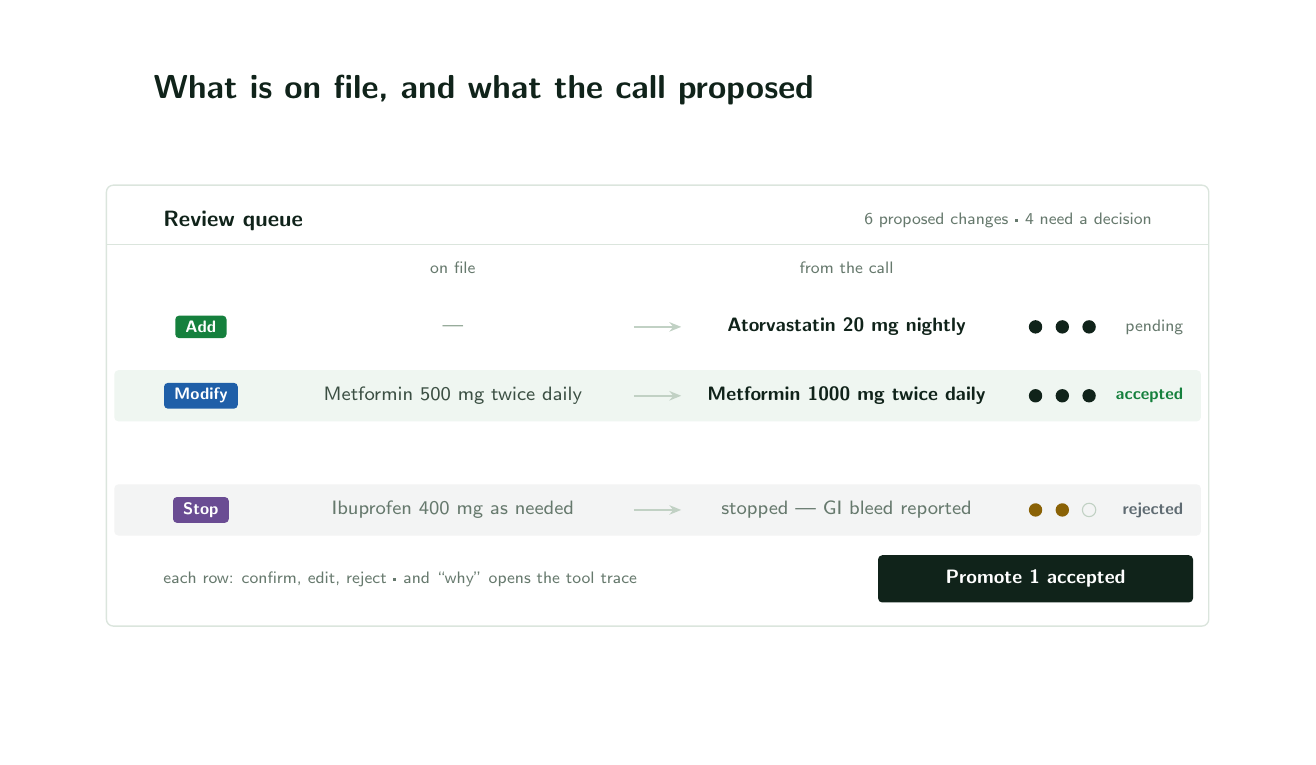
\begin{tikzpicture}[x=1mm,y=1mm]
\path[use as bounding box] (0,0) rectangle (160,90);

\node[headline] at (16,82) {What is on file, and what the call proposed};

% ---- the screen ---------------------------------------------------------
\fill[surf, rounded corners=2.5pt] (10,14) rectangle (150,70);
\draw[line, line width=0.5pt, rounded corners=2.5pt] (10,14) rectangle (150,70);

\node[anchor=west, font=\fontsize{8.5}{10}\selectfont\sffamily\bfseries\color{ink}] at (16,65.5) {Review queue};
\node[anchor=east, font=\fontsize{6.4}{7.5}\selectfont\sffamily\color{inkiii}] at (144,65.5) {6 proposed changes \textperiodcentered\ 4 need a decision};
\draw[line] (10,62.5) -- (150,62.5);

\node[anchor=center, font=\fontsize{6.2}{7}\selectfont\sffamily\color{inkiii}] at (54,59.5) {on file};
\node[anchor=center, font=\fontsize{6.2}{7}\selectfont\sffamily\color{inkiii}] at (104,59.5) {from the call};

% ---- rows ---------------------------------------------------------------
% row 1 — add, pending
\node[tag, fill=add, text=white, anchor=center] at (22,52) {Add};
\node[anchor=center, font=\fontsize{6.6}{8}\selectfont\sffamily\color{inkiv}] at (54,52) {\textemdash};
\draw[flow] (77,52) -- (83,52);
\node[anchor=center, font=\fontsize{6.6}{8}\selectfont\sffamily\bfseries\color{ink}] at (104,52) {Atorvastatin 20 mg nightly};
\foreach \i in {0,1,2}{\fill[ink] (128+\i*3.4,52) circle (0.85);}
\node[anchor=east, font=\fontsize{6.2}{7}\selectfont\sffamily\color{inkiii}] at (148,52) {pending};

% row 2 — modify, accepted
\fill[add!7!white, rounded corners=1.5pt] (11,40) rectangle (149,46.5);
\node[tag, fill=modify, text=white, anchor=center] at (22,43.25) {Modify};
\node[anchor=center, font=\fontsize{6.6}{8}\selectfont\sffamily\color{inkii}] at (54,43.25) {Metformin 500 mg twice daily};
\draw[flow] (77,43.25) -- (83,43.25);
\node[anchor=center, font=\fontsize{6.6}{8}\selectfont\sffamily\bfseries\color{ink}] at (104,43.25) {Metformin 1000 mg twice daily};
\foreach \i in {0,1,2}{\fill[ink] (128+\i*3.4,43.25) circle (0.85);}
\node[anchor=east, font=\fontsize{6.2}{7}\selectfont\sffamily\bfseries\color{accept}] at (148,43.25) {accepted};

% row 3 — stop, rejected
\fill[ink!5!white, rounded corners=1.5pt] (11,25.5) rectangle (149,32);
\node[tag, fill=stop, text=white, anchor=center] at (22,28.75) {Stop};
\node[anchor=center, font=\fontsize{6.6}{8}\selectfont\sffamily\color{inkiii}] at (54,28.75) {Ibuprofen 400 mg as needed};
\draw[flow] (77,28.75) -- (83,28.75);
\node[anchor=center, font=\fontsize{6.6}{8}\selectfont\sffamily\color{inkiii}] at (104,28.75) {stopped \textemdash\ GI bleed reported};
\foreach \i in {0,1}{\fill[caution] (128+\i*3.4,28.75) circle (0.85);}
\draw[lineii] (134.8,28.75) circle (0.85);
\node[anchor=east, font=\fontsize{6.2}{7}\selectfont\sffamily\bfseries\color{reject}] at (148,28.75) {rejected};

% ---- the one action -----------------------------------------------------
\fill[ink, rounded corners=1.5pt] (108,17) rectangle (148,23);
\node[anchor=center, font=\fontsize{6.6}{8}\selectfont\sffamily\bfseries\color{white}] at (128,20) {Promote 1 accepted};
\node[anchor=west, font=\fontsize{6.2}{7}\selectfont\sffamily\color{inkiii}] at (16,20)
  {each row: confirm, edit, reject \textperiodcentered\ and \textquotedblleft why\textquotedblright\ opens the tool trace};

\end{tikzpicture}
\end{document}
